\chapter{Automatic differentiation}
\label{chap:automatic_differentiation}

\begin{supportbox}{About this chapter}
The previous chapter highlighted the need for an efficient, automatic procedure to compute gradients of any possible sequence of operations. In this chapter we describe such a method, called \textbf{back-propagation} in the neural network’s literature or \textbf{reverse-mode automatic differentiation} in the computer science one. Its analysis has several insights, ranging from the model's choice to the memory requirements for optimizing it.
\end{supportbox}

\section{Problem setup}

We consider the problem of efficiently computing gradients of generic \textit{computational graphs}, such as those induced by optimizing a scalar loss function on a fully-connected model, a task called \textbf{automatic differentiation} (AD) \cite{baydin2018automatic}. You can think of a computational graph as the set of atomic operations (which we call \textbf{primitives}) obtained by running the program itself. We will consider sequential graphs for brevity, but everything can be easily extended to acyclic and even more generic computational graphs \cite{griewank2008evaluating,blondel2024elements} .

The problem may seem trivial, since the chain rule of Jacobians (Section \ref{sec:gradients_and_jacobians}, \eqref{eq:jacobian_chain_rule}) tells us that the gradient of function composition is simply the matrix product of the corresponding Jacobian matrices. However, efficiently implementing this is the key challenge, and the resulting algorithm (\textbf{reverse-mode AD} or \textbf{backpropagation}) is a cornerstone of neural networks and differentiable programming in general \cite{griewank2008evaluating,blondel2024elements}. Understanding it is also key to understanding the design (and the differences) of most frameworks for implementing and training such programs (such as TensorFlow or PyTorch or JAX). A brief history of the algorithm can be found in \cite{griewank2012invented}.

To setup the problem, we assume we have at our disposal a set of \textbf{primitives}:
%
$$
\mathbf{y} =f_i(\mathbf{x}, \mathbf{w}_i)
$$
%
Each primitive represents an operation on an input vector $\mathbf{x} \sim ({c_i})$, parameterized by the vector $\mathbf{w}_i \sim (p_i)$ (e.g., the weights of a linear projection), and giving as output another vector $\mathbf{y} \sim (c^\prime_i)$.

There is a lot of flexibility in our definition of primitives, which can represent basic linear algebra operations (e.g., matrix multiplication), layers in the sense of Chapter \ref{chap:fully_connected_models} (e.g., a fully-connected layer with an activation function), or even larger blocks or models. This recursive composability is a key property of programming and extends to our case.

We only assume that for each primitive we know how to compute the partial derivatives with respect to the two input arguments, which we call the \textbf{input Jacobian} and the \textbf{weight Jacobian} of the operation:
%
\begin{eqnarray*}
\textbf{Input Jacobian: } & \partial_{\mathbf{x}}\left[f(\mathbf{x},\mathbf{w})\right] \sim (c^\prime,c) \\ 
\textbf{Weight Jacobian: } & \partial_{\mathbf{w}}\left[f(\mathbf{x},\mathbf{w})\right] \sim (c^\prime,p) 
\end{eqnarray*}

These are reasonable assumptions since we restrict our analysis to differentiable models. Continuous primitives with one or more points of non-differentiability, such as the ReLU, can be made to fit into this framework with the use of \textbf{subgradients} (Section \ref{subsec:subdifferentiability}). Non differentiable operations such as sampling or thresholding can also be included by finding a relaxation of their gradient or an equivalent estimator \cite{niculae2023discrete}. We cover the latter case in the next volume.
%
\subsection*{On our notation and higher-order Jacobians}

\addteacup We only consider vector-valued quantities for readability, as all resulting gradients are matrices. In practice, existing primitives may have inputs, weights, or outputs of higher rank. For example, consider a basic fully-connected layer on a mini-batched input:
%
$$
f(\mathbf{X},\mathbf{W})=\mathbf{X}\mathbf{W}+\mathbf{b}
$$
%
In this case, the input $\mathbf{X}$ has shape $(n,c)$, the weights have shape $(c,c’)$ and $(c^\prime)$ (with $c^\prime$ a hyper-parameter), and the output has shape $(n, c^\prime)$. Hence, the input Jacobian has shape $(n,c^\prime, n, c)$, and the weight Jacobian has shape $(n,c^\prime, c, c^\prime)$, both having rank $4$. 

In our notation, we can consider the equivalent flattened vectors $\mathbf{x} = \text{vect}(\mathbf{X})$ and $\mathbf{w} = \left[\text{vect}(\mathbf{W}); \mathbf{b}\right]$, and our resulting “flattened” Jacobians have shape $(nc^\prime, nc)$ and $(nc^\prime, cc^\prime)$ respectively. This is crucial in the following, since every time we refer to “\textit{the input size $c$}” we are referring to “\textit{the product of all input shapes}”, including eventual mini-batching dimensions. This also shows that, while we may know how to compute the Jacobians, we may not wish to fully \textit{materialize} them in memory due to their large dimensionality.

As a final note, our notation aligns with the way these primitives are implemented in a functional library, such as JAX. In an object-oriented framework (e.g., TensorFlow, PyTorch), we saw
that layers are implemented as objects (see Box \ref{code:fully_connected_layer} in the previous chapter), with the parameters being a property of the object, and the function call being replaced by an object’s method. This style simplifies certain practices, such as deferred initialization of all parameters until the input shapes are known (\textbf{lazy initialization}), but it adds a small layer of abstraction to consider to translate our notation into workable code. As we will see, these differences are reflected in turn in the way AD is implemented in the two frameworks.

\subsection{Automatic differentiation: problem statement}

With all these details out of the way, we are ready to state the AD task. Consider a sequence of $l$ primitive calls, followed by a final summation:
%
\begin{eqnarray*}
\mathbf{h}_1 & = & f_1(\mathbf{x}, \mathbf{w}_1) 
\\ \mathbf{h}_2 & = & f_2(\mathbf{h}_1, \mathbf{w}_2) \\ 
& \vdots &  \\ 
\mathbf{h}_{l} & = & f_{l}(\mathbf{h}_{l-1}, \mathbf{w}_{l}) 
\\ y & = & \sum \mathbf{h}_{l} 
\end{eqnarray*}
%
This is called an \textbf{evaluation trace} of the program. Roughly, the first $l-1$ operations can represent several layers of a differentiable model, operation $l$ can be a per-input loss (e.g., cross-entropy), and the final operation sums the losses of the mini-batch. Hence, the output of our program is always a scalar, since we require it for numerical optimization. We abbreviate the previous program as $F(\mathbf{x})$. 

\begin{definition}[Automatic differentiation] \addbottle
%
Given a program $F(\mathbf{x})$ composed of a sequence of differentiable primitives, \textbf{automatic differentiation} (AD) refers to the task of \textit{simultaneously} and \textit{efficiently} computing all weight Jacobians of the program given knowledge of the computational graph and all individuals input and weight Jacobians:
%
$$
\text{AD}(F(\mathbf{x}))=\left\{\partial_{\mathbf{w}_i} y\right\}_{i=1}^{l}
$$
\end{definition}
%
As we will see, there are two major classes of AD algorithms, called \textbf{forward-mode} and \textbf{backward-mode}, corresponding to a different ordering in the composition of the individual operations. We will also see that the backward-mode (called \textbf{back-propagation} in the neural networks’ literature) is significantly more efficient in our context. While we focus on a simplified scenario, it is relatively easy to extend our derivation to acyclic graphs of primitives (as already mentioned), and also to situations where parameters are shared across layers (\textbf{weight sharing}). We will see an example of weight sharing in Chapter \ref{chap:rnns}.

\subsection{Numerical and symbolic differentiation}

\addteacup Before moving on to forward-mode AD, we comment on the difference between AD and other classes of algorithms for differentiating functions. First, we could directly apply the definition of gradients (Section \ref{sec:gradients_and_jacobians}) to obtain a suitable numerical approximation of the gradient. This process is called \textbf{numerical differentiation}. However, each scalar value to be differentiated requires $2$ function calls in a naive implementation, making this approach unfeasible except for numerical checks over the implementation.

Second, consider this simple function:
%
$$
f(x)=a\sin(x)+bx\sin(x)
$$
%
We can ask a symbolic engine to pre-compute the full, symbolic equation of the derivative. This is called \textbf{symbolic differentiation} and shown in Python in Box \ref{code:symbolic_differentiation}.

In a realistic implementation, the intermediate value $h=\sin(x)$ would be computed only once and stored in an intermediate variable, which can also be reused for the corresponding computation in the gradient trace (and a similar reasoning goes for the $\cos(x)$ term in the derivative). This is less trivial than it appears: finding an optimal implementation for the Jacobian which avoids any unnecessary computation is an NP-complete task (\textbf{optimal Jacobian accumulation}). However, we will see that we can exploit the structure of our program to devise a suitably efficient implementation of AD that is significantly better than a symbolic approach like the above (and it is, in fact, equivalent to a symbolic approach allowing for the presence of subsequences \cite{laue2019equivalence}).

\begin{mypy}{Symbolic differentiation in Python using SymPy.}{code:symbolic_differentiation}
import sympy as sp
x, a, b = sp.symbols('x a b')
y = a*sp.sin(x) + b*x*sp.sin(x)
sp.diff(y, x) # [Out]: acos(x)+bxcos(x)+bsin(x)
\end{mypy}

\section{Forward-mode automatic differentiation}

We begin by recalling the chain rule of Jacobians. Consider a combination of two primitive functions:
%
$$
\mathbf{h}=f_1(\mathbf{x)} \;,\; \mathbf{y}=f_2(\mathbf{h})
$$
%
In terms of their gradients, we have:
%
$$
\partial_{\mathbf{x}}\,\mathbf{y} = {\color{drawgreen}\partial_{\mathbf{h}} \,\mathbf{y}} \,\cdot\,{\color{drawred}\partial_{\mathbf{x}}\,\mathbf{h}}
$$
%
If $\mathbf{x}$, $\mathbf{h}$, and $\mathbf{y}$ have dimensions $a$, $b$, and $c$ respectively, the previous Jacobian requires the multiplication of a $c \times b$ matrix (in green) with a $b \times a$ one (in red). We can interpret the rule as follows: if we have already computed $f_1$ and its Jacobian (red term), once we apply $f_2$ we can “update” the gradient by multiplying with the corresponding Jacobian (green term).

We can immediately apply this insight to obtain a working algorithm called \textbf{forward-mode automatic differentiation} (F-AD). The idea is that every time we apply a primitive function, we initialize its corresponding weight Jacobian (called \textbf{tangent} in this context), while simultaneously updating all previous tangent matrices. Let us see a simple worked-out example to illustrate the main algorithm.

Consider the first instruction, $\mathbf{h}_1 = f_1(\mathbf{x}, \mathbf{w}_1)$, in our program. Because nothing has been stored up to now, we initialize the tangent matrix for $\mathbf{w}_1$ as its weight Jacobian:

$$
\widehat{\mathbf{W}}_1 = \partial_{\mathbf{w}_1} \, \mathbf{h}_1
$$

We now proceed to the second instruction, $\mathbf{h}_2 = f_2(\mathbf{h}_1, \mathbf{w}_2)$. We update the previous tangent matrix while simultaneously initializing the second one:

\begin{gather*}
\eqnmarkbox[drawgreen]{node2}{\widehat{\mathbf{W}}_1} \leftarrow \eqnmarkbox[drawred]{node}{\left[\partial_{\mathbf{h}_1} \mathbf{h}_2\right]} \widehat{\mathbf{W}}_1 \\
\widehat{\mathbf{W}}_2 = \partial_{\mathbf{w}_2}\,\mathbf{h}_2
\end{gather*}
\annotate[yshift=1em]{above,right}{node}{Input Jacobian of $f_2$}
\annotate[yshift=1em]{above,left}{node2}{Updated tangent matrix for $\mathbf{w}_1$}

\vspace{-2em}
The update requires the input Jacobian of the primitive, while the second term requires the weight Jacobian of the primitive. Abstracting away, consider the generic $i$-th primitive given by $\mathbf{h}_i = f_i(\mathbf{h}_{i-1}, \mathbf{w}_i)$. We initialize the tangent matrix for $\mathbf{w}_i$ while simultaneously updating \textit{all} previous matrices:

\begin{gather*}
\widehat{\mathbf{W}}_j \leftarrow \left[\eqnmarkbox[drawred]{node}{\partial_{\mathbf{h}_{i-1}} \mathbf{h}_i}\right] \widehat{\mathbf{W}}_j \;\; \forall j <i \\
\widehat{\mathbf{W}}_i = \eqnmarkbox[drawgreen]{node2}{\partial_{\mathbf{w}_i}}\,\mathbf{h}_i
\end{gather*}
\annotate[yshift=1em]{above,right}{node}{Input Jacobian of $f_i$}
\annotate[yshift=-1em]{below,right}{node2}{Weight Jacobian of $f_i$}

\vspace{1em}
There are $i-1$ updates in the first row (one for each tangent matrix we have already stored in memory), with the red term -- the input Jacobian of the $i$-th operation -- being shared for all previous tangents. The last operation in the program is a sum, and the corresponding gradient gives us the output of the algorithm:\footnote{To be fully consistent with notation, the output of \eqref{eq:last_step_fad} is a row vector, while we defined the gradient as a column vector. We will ignore this subtle point for simplicity until it is time to define vector-Jacobian products later on the in the chapter.}

\begin{equation}
\nabla_{\mathbf{w}_i}y=  \mathbf{1}^\top\widehat{\mathbf{W}}_i \;\; \forall i
\label{eq:last_step_fad}
\end{equation}

Done! Let us analyze the algorithm in more detail. First, all the operations we listed can be easily \textit{interleaved} with the original program, meaning that the space complexity will be roughly proportional to the space complexity of the program we are differentiating.

On the negative side, the core operation of the algorithm (the update of $\widehat{\mathbf{W}}_i$) requires a multiplication of two matrices, generically shaped $(c^\prime_i, c_i)$ and $(c_i, p_j)$, where $c_i, c^\prime_i$ are input/output shapes, and $p_j$ is the shape of $\mathbf{w}_j$. This is an extremely expensive operation: for example, assume that inputs and outputs are both shaped $(n,d)$, where $n$ is the mini-batch dimension and $d$ represents the input/output features. Then, the matrix multiplication will have complexity $\mathcal{O}(n^2d^2p_j)$, which is quadratic in both mini-batch size and feature dimensionality. This can easily become unfeasible, especially for high-dimensional inputs such as images.

We can obtain a better trade-off by noting that the last operation of the algorithm is a simpler matrix-vector product, which is a consequence of having a scalar output. This is explored in more detail in the next section.

\section{Reverse-mode automatic differentiation}
\label{sec:reverse_mode_automatic_differentiation}

\addclock To proceed, we unroll the computation of a single gradient term corresponding to the $i$-th weight matrix:
%
\begin{equation}
\nabla_{\mathbf{w}_i}\,y = \mathbf{1}^\top {\color{drawred}\left[ \partial_{\mathbf{h}_{l-1}}\,\mathbf{h}_{l}\right] \cdots \left[ \partial_{\mathbf{h}_{i}}\,\mathbf{h}_{i+1}\right]} {\color{drawgreen}\left[ \partial_{\mathbf{w}_{i}}\,\mathbf{h}_{i}\right]}
\label{eq:backward_pass}
\end{equation}
%
Remember that, notation apart, \eqref{eq:backward_pass} is just a potentially long series of matrix multiplications, involving a constant term (a vector $\mathbf{1}$ of ones), a series of input Jacobians (the red term) and a weight Jacobian of the corresponding weight matrix (the green term). Let us define a shorthand for the red term:
%
\begin{equation}
    \widetilde{\mathbf{h}}_i = \mathbf{1}^\top \prod_{j=i+1}^{l} \partial_{\mathbf{h}_{j-1}}\,\mathbf{h}_{j}
    \label{eq:recursive_h}
\end{equation}
%
Because matrix multiplication is associative, we can perform the computations in \eqref{eq:backward_pass} in any order. In F-AD, we proceeded from the right to the left, since it corresponds to the ordering in which the primitive functions were executed. However, we can do better by noting two interesting aspects:

\begin{enumerate}
\item The leftmost term in \eqref{eq:backward_pass} is a product between a vector and a matrix (which is a consequence of having a scalar term in output), which is computationally better than a product between two matrices. Its output is also another vector.
\item The term in \eqref{eq:recursive_h} (the product of all input Jacobians from layer $i$ to layer $l$) can be computed recursively starting from the \textit{last} term and iteratively multiplying by the input Jacobians in the reverse order.
\end{enumerate}

We can put together these observations to develop a second approach to automatic differentiation, that we call \textbf{reverse-mode automatic differentiation} (R-AD), which is outlined next.

\begin{enumerate}
\item Differently from F-AD, we start by executing the \textit{entire} program to be differentiated, storing all intermediate outputs.
\item We inizialize a vector $\widetilde{\mathbf{h}} =\mathbf{1}^\top$, which corresponds to the leftmost term in \eqref{eq:backward_pass}.
\item Moving in reverse order, i.e., for an index $i$ ranging in $l, l-1, l-2,\ldots, 1$, we first compute the gradient with respect to the $i$-th weight matrix as:
%
$$
\partial_{\mathbf{w}_i}\, y  = \widetilde{\mathbf{h}} \left[\partial_{\mathbf{w}_i} \mathbf{h}_{i}\right]
$$
%
which is the $i$-th gradient we need. Next, we update our “back-propagated” input Jacobian as:
%
$$
\widetilde{\mathbf{h}} \leftarrow \widetilde{\mathbf{h}} \left[\partial_{\mathbf{h}_{i-1}}\mathbf{h}_{i}\right]
$$
\end{enumerate}

Steps (1)-(3) describe a program which is roughly symmetrical to the original program, that we call the \textbf{dual} or \textbf{reverse} program. The terms $\widetilde{\mathbf{h}}$ are called the \textbf{adjoints} and they store (sequentially) all the gradients of the output with respect to the variables $\mathbf{h}_1, \mathbf{h}_2, \ldots, \mathbf{h}_{l}$ in our program.\footnote{Compare this with F-AD, where the tangents represented instead the gradients of the $\mathbf{h}_i$ variables with respect to the weights.}

In the terminology of neural networks, we sometimes say that the original (\textbf{primal}) program is a \textbf{forward pass} (not to be confused with forward-mode), while the reverse program is a \textbf{backward pass}. Differently from F-AD, in R-AD the full primal program must be executed before the reverse program can be run, and we need specialized mechanisms to store all intermediate outputs to “unroll” the computational graph. Different frameworks implement this differently, as outlined next.

Computationally, R-AD is significantly more efficient than F-AD. In particular, both operations in step (3) of R-AD are vector-matrix products scaling only linearly in all shape quantities. The tradeoff is that executing R-AD requires a large amount of memory, since all intermediate values of the primal program must be stored on disk with a suitable strategy. Specific techniques, such as \textbf{gradient checkpointing}, can be used to improve on this tradeoff by increasing computations and partially reducing the memory requirements. This is done by only storing a few intermediate outputs (called \textbf{checkpoints}) while recomputing the remaining values during the backward pass. See Figure \ref{fig:gradient_checkpointing} for a visualization.

\begin{figure}
    \centering
    \begin{subfigure}[b]{0.23\textwidth}
    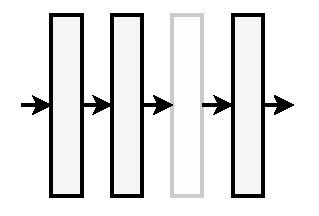
\includegraphics[width=1.0\textwidth]{images/gradient_checkpointing-Pagina-1}
    \caption{}
    \end{subfigure}
    \hfill
    \begin{subfigure}[b]{0.23\textwidth}
    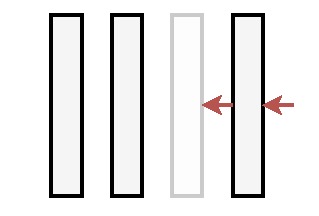
\includegraphics[width=1.0\textwidth]{images/gradient_checkpointing-Pagina-2}
    \caption{}
    \end{subfigure}
    \hfill
    \begin{subfigure}[b]{0.23\textwidth}
    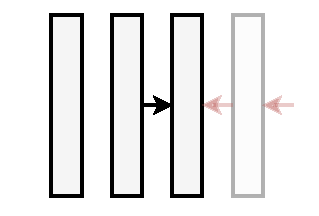
\includegraphics[width=1.0\textwidth]{images/gradient_checkpointing-Pagina-3}
    \caption{}
    \end{subfigure}
    \hfill
    \begin{subfigure}[b]{0.23\textwidth}
    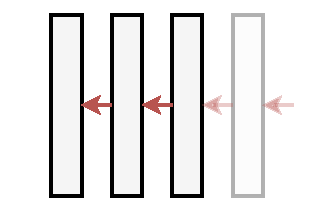
\includegraphics[width=1.0\textwidth]{images/gradient_checkpointing-Pagina-4}
    \caption{}
    \end{subfigure}
    \hfill
    \caption{An example of \textbf{gradient checkpointing}. (a) We execute a forward pass, but we only store the outputs of the first, second, and fourth blocks (\textbf{checkpoints}). (b) The backward pass (red arrows) stops at the third block, whose activations are not available. (c) We run a second forward pass starting from the closest checkpoint to materialize again the activations. (d) We complete the forward pass. Compared to a standard backward pass, this requires 1.25x more computations. In general, the less checkpoints are stored, the higher the computational cost of the backward pass.}
    \label{fig:gradient_checkpointing}
\end{figure}

\section{Practical considerations}

\subsection{Vector-Jacobian products}

Looking at step (3) in the R-AD algorithm, we can make an interesting observation: the only operation we need is a product between a row vector $\mathbf{v}$ and a Jacobian of $f$ (either the input or the weight Jacobian). We call these two operations the \textbf{vector-Jacobian products} (VJPs) of $f$.\footnote{By contrast, F-AD can be formulated entirely in terms of the transpose of the VJP, called a \textbf{Jacobian-vector product} (JVP). For a one-dimensional output, the JVP is the directional derivative \eqref{eq:directional_derivative} from Section \ref{sec:gradients_and_jacobians}. Always by analogy, the VJP represents the application of a linear map connected to infinitesimal variations of the \textit{output} of the function, see \cite{blondel2024elements}.} In the next definition we restore dimensional consistency by adding a transpose to the vector.

\begin{definition}[Vector-Jacobian product (VJP)] \addbottle
    Given a function $\mathbf{y}=f(\mathbf{x})$, with $\mathbf{x} \sim (c)$ and $\mathbf{y} \sim (c^\prime)$, its VJP is another function defined as:
    %
    \begin{equation}
    \textnormal{vjp}_f(\mathbf{v})=\mathbf{v}^\top \partial f(\mathbf{x})
    \end{equation}
    %
    where $\mathbf{v}\sim (c^\prime)$. If $f$ has multiple parameters $f(\mathbf{x}_1, \ldots, \mathbf{x}_n)$, we can define $n$ individual VJPs denoted as $\textnormal{vjp}_{f,\mathbf{x}_1}(\mathbf{v})$, ..., $\textnormal{vjp}_{f, \mathbf{x}_n}(\mathbf{v})$.
\end{definition}

In particular, in our case we can define two types of VJPs, corresponding to the input and the weight argument respectively:
%
\begin{gather}
\text{vjp}_{f,\mathbf{x}}(\mathbf{v})=\mathbf{v}^\top\partial_\mathbf{x}f(\mathbf{x},\mathbf{w}) \label{eq:input_jacobian}\\ \text{vjp}_{f, \mathbf{w}}(\mathbf{v})=\mathbf{v}^\top\partial_\mathbf{w}f(\mathbf{x},\mathbf{w})\label{eq:weight_jacobian}
\end{gather}
%
We can now rewrite the two operations in step (3) of the R-AD algorithm as two VJP calls of the primitive function with the adjoint values (ignoring the $i$ indices for readability), corresponding to the adjoint times the weight VJP, and the adjoint times the input VJP:
%
\begin{gather}
\partial_{\mathbf{w}} \, y = \text{vjp}_{f,\mathbf{w}}\left(\widetilde{\mathbf{h}}\right) \label{eq:r_ad_1}\\ \widetilde{\mathbf{h}}  \gets \text{vjp}_{f, \mathbf{h}}\left(\widetilde{\mathbf{h}}\right) \label{eq:r_ad_2}
\end{gather}
%
Hence, we can implement an entire automatic differentiation system by first choosing a set of primitives operations, and then augmenting them with the corresponding VJPs, without having to materialize the Jacobians in memory at any point. This is shown schematically in Figure \ref{fig:backward_pass}. 

\begin{SCfigure}
    \centering
    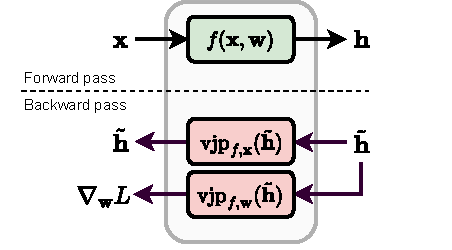
\includegraphics[width=0.55\textwidth]{images/backward_pass-Pagina-2.pdf}
    \caption{For performing R-AD, primitives must be augmented with two VJP operations to be able to perform a backward pass, corresponding to the input VJP \eqref{eq:input_jacobian} and the weight VJP \eqref{eq:weight_jacobian}. One call for each is sufficient to perform the backward pass through the primitive, corresponding to \eqref{eq:r_ad_1}-\eqref{eq:r_ad_2}.}
    \label{fig:backward_pass}
\end{SCfigure}

In fact, we can recover the Jacobians' computation by repeatedly calling the VJPs with the basis vectors $\mathbf{e}_1, \ldots, \mathbf{e}_n$, to generate them one row at a time, e.g., for the input Jacobian we have:
%
$$
\partial_{\mathbf{x}}f(\mathbf{x},\mathbf{w})=\begin{bmatrix} \text{vjp}_{f,\mathbf{x}}(\mathbf{e}_1) \\ \text{vjp}_{f,\mathbf{x}}(\mathbf{e}_2) \\ \vdots\\ \text{vjp}_{f,\mathbf{x}}(
\mathbf{e}_n) \end{bmatrix}
$$
%
To understand why this reformulation can be convenient, let us look at the VJPs of a fully-connected layer, which is composed of linear projections and (elementwise) non-linearities. First, consider a simple linear projection with no bias:
%
$$
f(\mathbf{x}, \mathbf{W})=\mathbf{W}\mathbf{x}
$$
%
The input Jacobian here is simply $\mathbf{W}$, but the weight Jacobian is a rank-3 tensor (Section \ref{sec:gradients_and_jacobians}). By comparison, the input VJP has no special structure:
%
\begin{equation}
\text{vjp}_{f, \mathbf{x}}(\mathbf{v})=\mathbf{v}^\top\mathbf{W}^\top = \left[\mathbf{W}\mathbf{v}\right]^\top
\label{eq:vjp_x_matrix_multiplication}
\end{equation}
%
The weight VJP, instead, turns out to be a simple outer product, which avoids rank-3 tensors completely:
%
\begin{equation}
\text{vjp}_{f,\mathbf{w}}(\mathbf{v}) = \mathbf{v}\mathbf{x}^\top
\label{eq:vjp_w_matrix_multiplication}
\end{equation}
%
\begin{supportbox}{Working out the VJP}
To compute \eqref{eq:vjp_w_matrix_multiplication}, we can write $y=\mathbf{v}^\top \mathbf{W}\mathbf{x} =\sum_i\sum_j W_{ij}v_ix_j$, from which we immediately get $\frac{\partial y}{\partial W_{ij}} = v_ix_j$, which is the elementwise definition of the outer product.
\end{supportbox}
%
Hence, every time we apply a linear projection in the forward pass, we modify the back-propagated gradients by the transpose of its weights, and we perform an outer product to compute the gradient of $\mathbf{W}$. 

Consider now an element-wise activation function with no trainable parameters, e.g., the ReLU:
%
$$
f(\mathbf{x},\left\{\right\})=\phi(\mathbf{x})
$$
%
Because we have no trainable parameters, we need only consider the input VJP. The gradient is a diagonal matrix having as elements the derivatives of $\phi$:
%
$$
\idx{\partial_{\mathbf{x}} \phi(\mathbf{x})}{ii}=\phi^\prime(x_i)
$$
%
The input VJP is a multiplication of a diagonal matrix by a vector, which is equivalent to an Hadamard product (i.e., a scaling operation):
%
\begin{equation}
\text{vjp}_{\mathbf{x}}(f,\mathbf{v})=\mathbf{v}\odot \phi^\prime(\mathbf{x})
\label{eq:backward_pass_activation_function}
\end{equation}
%
Interestingly, also in this case we can compute the VJP without having to materialize the full diagonal matrix.

\subsection{Implementing a R-AD system}
\label{subsec:implementing_rad}
%
There are many ways to implement the R-AD system, ranging form Wengert lists (as done in TensorFlow) to source-to-source code transformations \cite{griewank2008evaluating}. Here, we discuss briefly some common implementations in existing frameworks. 

First, describing primitives as functions with two arguments $f(\mathbf{x}, \mathbf{w})$ aligns with functional frameworks such as JAX, where everything is a function. Consider a function $f(\mathbf{x})$ with a $c$-dimensional input and a $c^\prime$-dimensional output. From this point of view, a VJP can be implemented as a higher-order function with signature:

\begin{mypy}{Gradient computation as a higher-order function. The \mintinline{python}{torch.func} interface replicates the JAX API. In practice, the function can be \textit{traced} (e.g., with {\footnotesize\mintinline{python}{torch.compile}}) to generate an optimized computational graph.}{code:functional_grad}
# Original function (sum-of-squares)
def f(x: Float[Array, "c"]):
  return (x**2).sum()

grad_f = func.grad(f)
print(grad_f(torch.randn(10)).shape) 
# [Out]: torch.Size([10])
\end{mypy}

\begin{equation}
(\mathbb{R}^c \rightarrow \mathbb{R}^{c^\prime}) \rightarrow \mathbb{R}^c \rightarrow (\mathbb{R}^{c^\prime} \rightarrow \mathbb{R}^c)
\end{equation}
%
i.e., given a function $f$ and an input $\mathbf{x}^\prime$, a VJP returns another function that can be applied to a $c^\prime$-dimensional vector $\mathbf{v}$ to return $\mathbf{v}^\top \partial f(\mathbf{x}^\prime)$. Similarly, the gradient for a one-dimensional function can be implemented as another higher-order function with signature:
%
\begin{equation}
(\mathbb{R}^c \rightarrow \mathbb{R}) \rightarrow (\mathbb{R}^c \rightarrow \mathbb{R}^c)
\end{equation}
%
taking as input the function $f(\mathbf{x})$ and returning another function that computes $\nabla f(\mathbf{x})$. In JAX, these ideas are implemented in the functions {\footnotesize\mintinline{python}{jax.grad}} and {\footnotesize\mintinline{python}{jax.jvp}} respectively, which is also replicated in PyTorch in the {\footnotesize\mintinline{python}{torch.func}} module - see Box \ref{code:functional_grad} for an example.\footnote{Many operations, such as computing an Hessian, can be achieved by smartly composing JVPs and VJPs based on their signatures: \url{https://jax.readthedocs.io/en/latest/notebooks/autodiff_cookbook.html}.}

As we mentioned, in practice our models are implemented as compositions of objects whose parameters are encapsulated as properties (Box \ref{code:fully_connected_layer}). One possibility is to ``purify'' the object to turn it into a pure function, e.g.:\footnote{\url{https://sjmielke.com/jax-purify.htm}}

{\footnotesize
\begin{minted}{python}
# Extract the parameters
params = dict(model.named_parameters())
# Functional call over the model's forward function
y = torch.func.functional_call(model, params, x)
\end{minted}
}

\begin{figure}
    \centering
    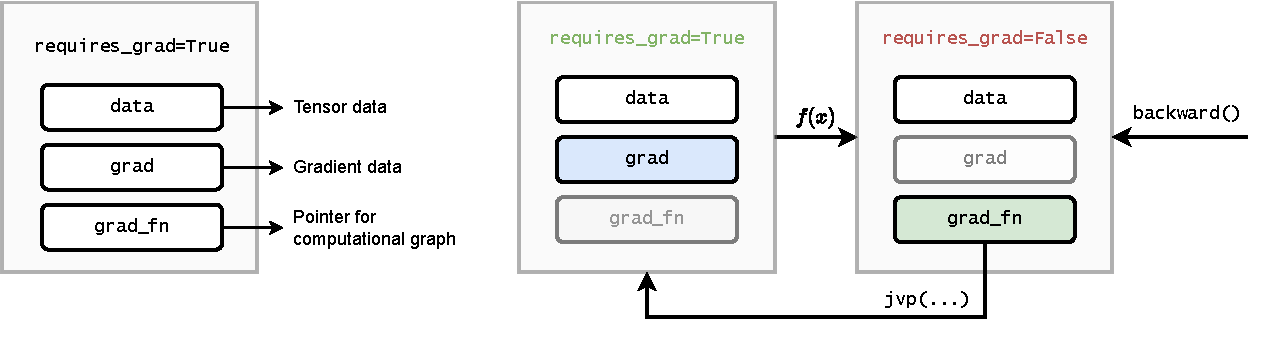
\includegraphics[width=\textwidth]{images/pytorch_wrapper-Pagina-2}
    \caption{Left: in PyTorch, a tensor is augmented with information about its gradient (empty at initialization), and about the operation that created it. Right: during a backward pass, the {\footnotesize\mintinline{python}{grad_fn}} property is used to traverse the computational graph in reverse, and gradients are stored \textit{inside} the tensor's {\footnotesize\mintinline{python}{grad}} property whenever {\footnotesize\mintinline{python}{requires_grad}} is explicitly set to {\footnotesize\mintinline{python}{True}} (to avoid consumming unnecessary memory).}
    \label{fig:pytorch_wrapper}
\end{figure}

More in general, frameworks like PyTorch are augmented with techniques to handle this scenario directly, without introducing intermediate operations. In PyTorch, for example, tensors' objects are augmented with information about the operation that generated them (Figure \ref{fig:pytorch_wrapper}, left). Whenever a {\footnotesize\mintinline{python}{backward()}} call is requested on a scalar value, these properties are used to traverse the computational graph in reverse, storing the corresponding gradients \textit{inside} the tensors that requires them (Figure \ref{fig:pytorch_wrapper}, right). 

This is just a high-level overview of how these systems are implemented in practice, and we are leaving behind many details, for which we refer to the official documentations.\footnote{I definitely suggest trying to implement an R-AD system from scratch: many didactical implementations can be found online, such as \url{https://github.com/karpathy/micrograd}.}

\subsection{Choosing an activation function}

Coincidentally, we can now motivate why ReLU is a good choice as activation function. A close look at \eqref{eq:backward_pass_activation_function} tells us that every time we add an activation function in our model, the adjoints in the backward pass are scaled by a factor of $\phi^\prime(\mathbf{x})$. For models with many layers, this can give rise to two pathological behaviors:

\begin{enumerate}
\item If $\phi^\prime(\cdot) < 1$ everywhere, there is the risk of the gradient being shrank to 0 exponentially fast in the number of layers. This is called the \textbf{vanishing gradient} problem.
\item Conversely, if $\phi^\prime(\cdot) > 1$ everywhere, the opposite problem appears, with the gradients exponentially converging to infinity in the number of layers. This is called the \textbf{exploding gradient} problem.
\end{enumerate}

These are serious problems in practice, because libraries represent floating point numbers with limited precision (typically 32 bits or lower), meaning that underflows or overflows can manifest quickly when increasing the number of layers.

\begin{supportbox}{Linear non-linear models}
Surprisingly, a stack of linear layers implemented in floating point precision is not fully linear because of small discontinuities at machine precision! This is generally not an issue, but it can be exploited to train fully-linear deep neural networks.\footnote{\url{https://openai.com/research/nonlinear-computation-in-deep-linear-networks}}
\end{supportbox}

As an example of how vanishing gradients can appear, consider the sigmoid function $\sigma(s)$. We already mentioned that this was a common AF in the past, due to it being a soft approximation to the step function. We also know that $\sigma^\prime(s)=\sigma(s)(1-\sigma(s))$. Combined with the fact that $\sigma(s) \in \left[0,1\right]$, we obtain that:
%
$$
\sigma^\prime(s)\in\left[0,0.25\right]
$$
%
Hence, the sigmoid is a prime candidate for vanishing gradient issues: see Figure \ref{fig:sigmoid_and_derivative}.

\begin{figure}
    \centering
    \begin{subfigure}[b]{0.48\textwidth}
    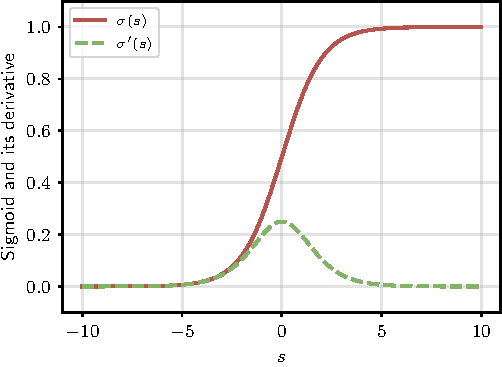
\includegraphics[width=1.0\textwidth]{images/sigmoid_and_derivative}
    \caption{Sigmoid}
    \label{fig:sigmoid_and_derivative}
    \end{subfigure}
    \hfill
    \begin{subfigure}[b]{0.48\textwidth}
    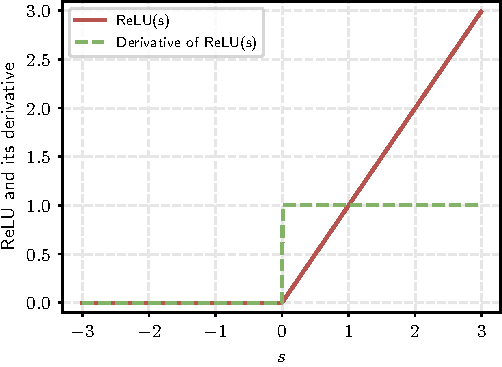
\includegraphics[width=1.0\textwidth]{images/relu_and_derivative}
    \caption{ReLU}
    \label{fig:relu_and_derivative}
    \end{subfigure}
    \caption{(a) Plot of the sigmoid function ({\color{drawred}red}) and its derivative ({\color{drawgreen}green}). (b) Plot of ReLU ({\color{drawred}red}) and its derivative ({\color{drawgreen}green}).}
\end{figure}

Designing an AF that never exhibits vanishing or exploding gradients is non trivial, since the only function having $\phi^\prime(s)=1$ everywhere is a constant function. We then need a function which is “linear enough” to avoid gradient issues, but “non-linear” enough to separate the linear layers. The ReLU ends up being a good candidate since:
%
$$
\partial_s \text{ReLU}(s)=\begin{cases} 0 & s < 0 \\ 1 & s >0 \end{cases}
$$
%
The gradient is either zeroed-out, inducing sparsity in the computation, or multiplied by $1$, avoiding scaling issues - this is shown in Figure \ref{fig:relu_and_derivative}.

As a side note, the ReLU’s gradient is identical irrespective of whether we replace the input to the ReLU layer with its output (since we are only masking the negative values while keeping the positive values untouched). Hence, another benefit of using ReLU as activation function is that we can save a small bit of memory when performing R-AD, by overwriting the layer’s input in the forward pass without impacting the correctness of the AD procedure: this is done in PyTorch, for example, by setting the {\footnotesize\verb+in_place+} parameter.\footnote{\url{https://pytorch.org/docs/stable/generated/torch.nn.ReLU.html}}

\subsection{Subdifferentiability and correctness of AD}
\label{subsec:subdifferentiability}

\addteacup There is a small detail we avoided discussing until now: the ReLU is non-differentiable in $0$, making the overall network non-smooth. What happens in this case? The “pragmatic” answer is that, by minimizing with stochastic gradient descent from a random (non-zero) initialization, the probability of ending up exactly in $s=0$ is practically null, while the gradient is defined in $\text{ReLU}(\varepsilon)$ for any $\lvert\varepsilon\rvert>0$.

For a more technical answer, we can introduce the concept of \textbf{subgradient} of a function.

\begin{definition}[Subgradient]
%
Given a convex function $f(x)$, a subgradient in $x$ is a point $z$ such that, for all $y$:
%
$$
f(y) \ge f(x)+z(y-x)
$$
%
\end{definition}

Note the similarity with the definition of convexity: a subgradient is the slope of a line “tangent” to $f(x)$, such that the entire $f$ is lower bounded by it. If $f$ is differentiable in $x$, then only one such line exists, which is the derivative of $f$ in $x$. In a non-smooth point, multiple subgradients exists, and they form a set called the \textbf{subdifferential} of $f$ in $x$:
%
$$
\partial_x f(x)=\left\{z \,\vert\, z \text{ is a subgradient of } f(x)\right\}
$$

With this definition in hand, we can complete our analysis of the gradient of ReLU by replacing the gradient with its subdifferential in $0$:
%
$$
\partial_s \text{ReLU}(s)=\begin{cases} \left\{0\right\} & s < 0 \\ \left\{1\right\} & s >0 \\ \left[0,1\right] & s=0 \end{cases}
$$
%
Hence, any value in $[0,1]$ is a valid subgradient in $0$, with most implementations in practice favoring $\text{ReLU}^\prime(0)=0$. Selecting subgradients at every step of an iterative descent procedure is called \textbf{subgradient descent}. 

In fact, the situation is even more tricky, because the subgradient need not be defined for non-convex functions. In that case, one can resort to generalizations that relax the previous definition to a local neighborhood of $x$, such as the Clarke subdifferential.\footnote{\url{https://en.wikipedia.org/wiki/Clarke_generalized_derivative}} Subdifferentiability can also create problems in AD, where different implementations of the same functions can provide different (possibly invalid) subgradients, and more refined concepts of chain rules must be considered for a formal proof \cite{kakade2018provably,bolte2020mathematical}.\footnote{Consider this example reproduced from \cite{bolte2020mathematical}: define two functions, $\text{ReLU}_2(s) = \text{ReLU}(-s)+s$ and $\text{ReLU}_3(s) = 0.5(\text{ReLU}(s)+\text{ReLU}_2(s))$. They are both equivalent to ReLU, but in PyTorch a backward pass in $0$ returns $0.0$ for ReLU, $1.0$ for ReLU$_2$, and $0.5$ for ReLU$_3$.}

\section*{From theory to practice}

\begin{wrapfigure}{r}{3.0cm}
\vspace{-3em}
\includegraphics[width=3.0cm]{images/shutterstock_2075221579.jpg}
\vspace{-3em}
\end{wrapfigure}

If you followed the exercises in Chapter \ref{chap:fully_connected_models}, you already saw an application of R-AD in both PyTorch and JAX, and this chapter (especially Section \ref{subsec:implementing_rad}) should have clarified their implementation.

It is a good idea to try and re-implement a simple R-AD system, similar to the one of PyTorch. For example, focusing on scalar-valued quantities, the \texttt{micrograd} repository\footnote{\url{https://github.com/karpathy/micrograd}} is a very good didactical implementation. The only detail we do not cover is that, once you move to a general acyclic graph, an ordering of the variables in the computational graph before the backward pass is essential to avoid creating wrong backpropagation paths. In micrograd, this is achieved via a non-expensive topological sorting of the variables.

It is also interesting to try and implement a new primitive (in the sense used in this chapter) in PyTorch, which requires specifying its forward pass along with its JVPs.\footnote{\url{https://pytorch.org/docs/master/notes/extending.html}} One example can be one of the trainable activation functions from Section \ref{sec:activation_functions}. This is a didactical exercise, in the sense that this can be implemented equivalently by subclassing \mintinline{python}{nn.Module} and letting PyTorch's AD engine work out the backward pass.

All these steps can also be replicated in JAX:
\begin{itemize}
\item Implement a didactic version of JAX with \texttt{autodidax}: \url{https://jax.readthedocs.io/en/latest/autodidax.html}
\item Write out a new primitive by implementing the corresponding VJP: \url{https://jax.readthedocs.io/en/latest/notebooks/Custom_derivative_rules_for_Python_code.html}
\item Read the \textbf{JAX Autodiff} Cookbook\footnote{\url{https://jax.readthedocs.io/en/latest/notebooks/autodiff_cookbook.html}} to discover advanced use-cases for the automatic differentiation engine, such as higher-order derivatives, Hessians, and more. 
\end{itemize}